\documentclass{article}
\usepackage{amsmath}
\usepackage{graphicx}
\usepackage{hyperref}
\usepackage{physics}
\usepackage[utf8]{inputenc}
\usepackage[dvipsnames]{xcolor}
\graphicspath{ {images/} }

\title{Homework 1}
\author{Lev Kozlov}
\date{September 2022}

\begin{document}

\maketitle

Source: \href{https://github.com/lvjonok/f22-theoretical-mechanics/tree/master/homework1}{Github repository}

\section{Task 1}

\href{https://github.com/lvjonok/f22-theoretical-mechanics/blob/master/homework1/motion_task1.gif}{Simulation link}

Solution:

We can start by calculating $y(x)$ from given parametric equations:

% write equations x = 3t, y = 4t^2 + 1

\begin{align}
    \vec{r}(t) & = \begin{bmatrix}
        3t \\
        4t^2 + 1
    \end{bmatrix}
\end{align}

Convert through expressing $t$ in terms of $x$ and substituting to $y$:

\begin{align}
    t = \frac{1}{3}x                        \\
    y(x) = 4\left(\frac{1}{3}x\right)^2 + 1 \\
    y(x) = \frac{4}{9}x^2 + 1
\end{align}

Calculating velocity and acceleration can be done through differentiation:

\begin{align}
    \frac{dr}{dt}(t) = \vec{v}(t) = \begin{bmatrix}
        3 \\
        8t
    \end{bmatrix}
\end{align}

\begin{align}
    v(t) = \sqrt{3^2 + 8^2t^2} = \sqrt{9 + 64t^2}
\end{align}

\begin{align}
    \frac{dv}{dt}(t) = \vec{a}(t) = \begin{bmatrix}
        0 \\
        8
    \end{bmatrix}
\end{align}

\begin{align}
    a(t) = \sqrt{0^2 + 8^2} = 8
\end{align}

Tangential acceleration can be calculating by taking the dot product of velocity and acceleration:

\begin{align}
    a_t(t) = || \vec{v}(t) || \cdot || \vec{a}(t) || = \
    \begin{bmatrix}
        0 \\
        8
    \end{bmatrix} \cdot \
    \begin{bmatrix}
        3 \\
        8t
    \end{bmatrix} * \frac{1}{\sqrt{9 + 64t^2}} = \
    \frac{64t}{\sqrt{9 + 64t^2}}
\end{align}

Simulation hint: we can find vectorized tangential acceleration by multiplying unit vector of velocity by scalar value of acceleration:

\begin{align}
    \vec{a}_t(t) = \frac{1}{|| \vec{v}(t) ||} \cdot \vec{v}(t) \cdot a_t(t) = \
    \frac{64t}{9 + 64t^2} \cdot \
    \frac{1}{\sqrt{9 + 64t^2}} \cdot \begin{bmatrix}
        3 \\
        8t
    \end{bmatrix}
\end{align}

Normal acceleration is simply the difference between acceleration and tangential acceleration:

\begin{align}
    \vec{a}_n(t) = \vec{a}(t) - \vec{a}_t(t)
\end{align}

But for usual calculation without simulation we could do it this way, by taking the cross product of velocity and acceleration:

\begin{align}
    \vec{a}_n(t) = \frac{|| \vec{v}(t) \times \vec{a}(t) ||}{v(t)} = \
    || \begin{bmatrix}
        3 \\
        8t
    \end{bmatrix} \times \
    \begin{bmatrix}
        0 \\
        8
    \end{bmatrix} || \
    \cdot \frac{1}{\sqrt{9 + 64t^2}} = \\
    || \begin{bmatrix}
        0 \\
        0 \\
        -24t
    \end{bmatrix} || \
    \cdot \frac{1}{\sqrt{9 + 64t^2}} = \
    \frac{24t}{\sqrt{9 + 64t^2}}
\end{align}

We can find curvature using this formula:

\begin{align}
    k(t) = \frac{a_n}{v(t)^2} = \
    \frac{24t}{\sqrt{9 + 64t^2}} \cdot \
    \frac{1}{9 + 64t^2} =
    \frac{24t}{(9 + 64t^2)^\frac{3}{2}}
\end{align}

\colorbox{green}{Answer:}

\begin{enumerate}
    \item \colorbox{green}{$y(x) = \frac{4}{9}x^2 + 1$}
    \item \colorbox{green}{$\vec{v(t)} = \begin{bmatrix}
                      3 \\
                      8t
                  \end{bmatrix}$}
    \item \colorbox{green}{$\vec{a(t)} = \begin{bmatrix}
                      0 \\
                      8
                  \end{bmatrix}$}
    \item \colorbox{green}{$a_t(t) = \frac{64t}{\sqrt{9 + 64t^2}}$}
    \item \colorbox{green}{$a_n(t) = \frac{24t}{\sqrt{9 + 64t^2}}$}
    \item \colorbox{green}{$k(t) = \frac{24t}{(9 + 64t^2)^\frac{3}{2}}$}
\end{enumerate}

\newpage

\section{Task 2}

\href{https://github.com/lvjonok/f22-theoretical-mechanics/blob/master/homework1/motion_task2.gif}{Simulation link}

Solution:

First of all I decided to change the coordinate system to make the problem easier. I will use the following coordinate system:

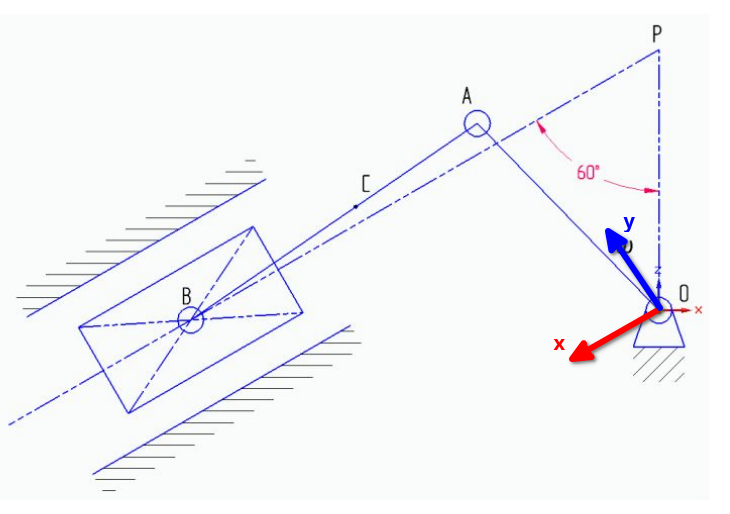
\includegraphics[width=\textwidth]{newcoordsystem.png}

Now we can describe point $B$ depending on input angle $\phi$:

\begin{align}
    B = \begin{bmatrix}
        PB - OP \cdot \cos{\frac{\pi}{3}} \\
        OP \cdot \cos{\frac{\pi}{3}}
    \end{bmatrix} = \
    OA \cdot \begin{bmatrix}
        \sin{(\phi)} \\
        \cos{(\phi)}
    \end{bmatrix} + \
    AB \cdot \begin{bmatrix}
        \sqrt{1 - \cos^2{(\gamma)}} \\
        \cos{(\gamma)}
    \end{bmatrix}
\end{align}

In this formula we have two unknowns: $\gamma$ and $PB$.
We can find $\gamma$ by using the fact that:
\begin{align}
    \cos{(\gamma)} = \frac{OP \cdot \cos{\frac{\pi}{3}} - OA \cos{\phi}}{AB}
\end{align}

Let me introduce very interesting fact:

\begin{align}
    \sin(arccos(x)) = \sqrt{1 - x^2}
\end{align}

Relax, won't bother you: \href{https://math.stackexchange.com/questions/345077/cos-arcsinx-sqrt1-x2-how}{explanation}

We are ready to calculate x coordinate of point $B$:

\begin{align}
    x_B = OA \cdot \sin{(\phi)} + AB \cdot \sin{(\gamma)}                                                         \\
    x_B = OA \cdot \sin{(\phi)} + AB \cdot \sqrt{1 - (\frac{OP \cdot \cos{\frac{\pi}{3}} - OA \cos{\phi}}{AB})^2} \\
    x_B = OA \cdot \sin{(\phi)} + \sqrt{AB^2 - (OP \cdot \cos{\frac{\pi}{3}} - OA \cos{\phi})^2}
\end{align}

That's it boom! We have found x coordinate of point $B$.

Velocity and acceleration will be simply calculated by differentiation of position
and I did it using online calculators. The only valuable information is that they have only x components.

Calculation of point C:

We know that point $C$ lies on the line $AB$ and we know that $AB = 80, AC = 20$.

So point $C$ is basically segment of line.

\begin{align}
    \vec{C} = \vec{A} + (\vec{B} - \vec{A}) \cdot \frac{AB}{AC}
\end{align}

Proportions will be the same for velocity and accelerations:

\begin{align}
    \vec{v_C} = \vec{v_A} + (\vec{v_B} - \vec{v_A}) \cdot \frac{AB}{AC} \\
    \vec{a_C} = \vec{a_A} + (\vec{a_B} - \vec{a_A}) \cdot \frac{AB}{AC}
\end{align}

Tangential acceleration is aligned with velocity vector:

\begin{align}
    \vec{a_{Ct}} = \vec{a_C} \cdot \frac{\vec{v_C}}{|| \vec{v_C} ||}
\end{align}

Normal acceleration is the difference between acceleration and tangential acceleration:

\begin{align}
    \vec{a_{Cn}} = \vec{a_C} - \vec{a_{Ct}}
\end{align}

That's it. We have found all the required values.

\colorbox{green}{Answer:}

\begin{enumerate}
    \item \colorbox{green}{$x_B(t) = OA \cdot \sin{(\phi)} + \sqrt{AB^2 - (OP \cdot \cos{\frac{\pi}{3}} - OA \cos{\phi})^2}$}
    \item \colorbox{green}{$v_B(t) = \dv{x_B(t)}{t}$}
    \item \colorbox{green}{$a_B(t) = \dv{v_B(t)}{t}$}
    \item \colorbox{green}{$\vec{C(t)} = \vec{A} + (\vec{B} - \vec{A}) \cdot \frac{AB}{AC}$}
    \item \colorbox{green}{$\vec{v_C(t)} = \vec{v_A} + (\vec{v_B} - \vec{v_A}) \cdot \frac{AB}{AC}$}
    \item \colorbox{green}{$\vec{a_C(t)} = \vec{a_A} + (\vec{a_B} - \vec{a_A}) \cdot \frac{AB}{AC}$}
\end{enumerate}

\newpage

\section{Task 3}

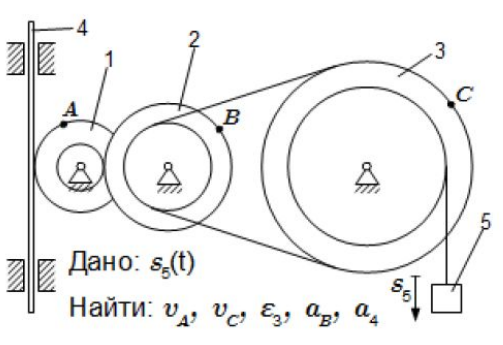
\includegraphics[width=\textwidth]{fig3.png}

Solution:

Given $s_5$ law of motion we can use it to propage through all the connections of the system:

Obviously, we can observe that point on inner $3_{rd}$ wheel will have the same speed.
Using this fact, we can get angular velocity of the $3_{rd}$ wheel:

\begin{align}
    \omega_3(t) = \frac{3t^2 - 6}{r_3}
\end{align}

Wheels 2 and 3 are connected using belt, so we can express angular velocity of the $2_{nd}$ wheel in terms of $3_{rd}$ wheel:

\begin{align}
    \omega_2(t) \cdot r_2 = \omega_3(t) \cdot R_3
\end{align}

The same idea between $1_{st}$ and $2_{nd}$ wheels is the same:

\begin{align}
    \omega_1(t) \cdot r_1 = \omega_2(t) \cdot R_2
\end{align}

These equations mainly give us everything to find required variables:

1. Velocity for point $A$ (on outer radius of the wheel $\implies$ uses $R_1$):

\begin{align}
    v_A(t) = \omega_1(t) \cdot R_1 = \frac{R_2}{r_1} \cdot \omega_2(t) \cdot {R_1} = \
    \frac{R_2}{r_1} \cdot \frac{R_3}{r_2} \cdot \omega_3(t) \cdot {R_1} = \notag \\
    \frac{R_2}{r_1} \cdot \frac{R_3}{r_2} \cdot \frac{3t^2 - 6}{r_3} \cdot {R_1}
\end{align}

At time $t = 2$ we have: $v_A(t) = \frac{8}{2} \cdot \frac{16}{6} \cdot \frac{6}{12} \cdot 4 = \frac{64}{3} \approx 21.33$

2. Velocity of point $C$ (on outer radius of the wheel $\implies$ uses $R_3$):

\begin{align}
    v_C(t) = \omega_3(t) \cdot R_3 = \frac{3t^2 - 6}{r_3} \cdot {R_3}
\end{align}

At time $t = 2$ we have: $v_C(t) = \frac{6}{12} \cdot 4 = \frac{24}{3} = 8$

3. Angular acceleration of $3_{rd}$ wheel.

\begin{align}
    \epsilon_3(t) = \dv{w_3(t)}{t} = \frac{6t}{r_3}
\end{align}

At time $t = 2$ we have: $\epsilon_3(t) = \frac{12}{12} = 1$

4. Acceleration of B:

We can start by determining angular speed and angular acceleration of the $2_{nd}$ wheel

\begin{align}
    \omega_2(t) = \frac{R_3}{r_2} \cdot \omega_3(t) = \frac{R_3}{r_2} \cdot \frac{3t^2 - 6}{r_3} \\
    \epsilon_2(t) = \dv{w_2(t)}{t} = \frac{R_3}{r_2} \cdot \epsilon_3(t) = \frac{R_3}{r_2} \cdot \frac{6t}{r_3}
\end{align}

Now we can apply basic transformations to find linear components of accelerations:

\begin{align}
    a_{B\tau}(t) = \epsilon_2(t) \times R_2 = \frac{R_3}{r_2} \cdot \frac{6t}{r_3} \cdot R_2              \\
    a_{Bn}(t) = \omega_2(t) \times ( \omega_2(t) \times R_2 ) = \
    \frac{R_3}{r_2} \cdot \frac{3t^2 - 6}{r_3} \cdot \frac{R_3}{r_2} \cdot \frac{3t^2 - 6}{r_3} \cdot R_2 \\
    a_{B}(t) = \sqrt{a_{B\tau}^2 + a_{Bn}^2}
\end{align}

At time $t = 2$ we have:

\begin{align}
    a_{B\tau}(2) = \frac{16}{6} \cdot \frac{12}{12} \cdot 8 = \frac{64}{3}                                    \\
    a_{Bn}(2) = \frac{16}{6} \cdot \frac{6}{12} \cdot \frac{16}{6} \cdot \frac{6}{12} \cdot 8 = \frac{128}{9} \\
    a_{B}(2) = \sqrt{\frac{64}{3}^2 + \frac{128}{9}^2} = 25.64
\end{align}

5. Acceleration of rack 4:

We see that it is connected without slippering to the $1_{st}$ wheel.
So we can express velocity of the bar in terms of angular velocity of the wheel:

\begin{align}
    v_{4}(t) = v_A(t) = \omega_1(t) \cdot R_1 = \frac{R_2}{r_1} \cdot \frac{R_3}{r_2} \cdot \frac{3t^2 - 6}{r_3} \cdot {R_1} \\
    a_{4}(t) = \dv{v_{4}(t)}{t} = \frac{R_2}{r_1} \cdot \frac{R_3}{r_2} \cdot \frac{6t}{r_3} \cdot {R_1}
\end{align}

At time $t = 2$ we have:

\begin{align}
    a_{4}(2) = \frac{8}{2} \cdot \frac{16}{6} \cdot \frac{12}{12} \cdot 4 = \frac{128}{3} = 42.67
\end{align}

\colorbox{green}{Answer:}

\begin{enumerate}
    \item \colorbox{green}{$v_A(2) = \frac{64}{3} \approx 21.33$}
    \item \colorbox{green}{$v_C(2) = 8$}
    \item \colorbox{green}{$\epsilon_3(2) = 1$}
    \item \colorbox{green}{$a_{B\tau}(2) = \frac{64}{3}$}
    \item \colorbox{green}{$a_{Bn}(2) = \frac{128}{9}$}
    \item \colorbox{green}{$a_{B}(2) = 25.64$}
    \item \colorbox{green}{$a_{4}(2) = 42.67$}
\end{enumerate}

\end{document}
